\subsection{Testprotokoll zu /LF03/}
\textbf{\hyperlink{lf-nn-01}{LF03}}

\subsubsection{Validierung der Sinnhaftigkeit der Merkmalsklassen}
Sie Sinnhaftigkeit und Relevanz der ausgewählten Merkmalsklassen wurden durch eine musikaffine Person, die gleichzeitig ein Gruppenmitglied ist, bestätigt.
Da die Relevanz der ausgewählten Merkmalsklassen für die Musikproduktion jedoch nicht sachlich sinnvoll in einem Testfall validiert werden kann, wird stattdessen die Fähigkeit zur Klassifizierung auf der Grundlage der auf einem Mikrocontroller verarbeitbaren Spektrogrammauflösung in die ausgewählten Merkmalsklassen betrachtet. Dabei wird ausschließlich die thoretische Umsetzbarkeit vor dem Training des neuronalen Netzes geprüft.

\paragraph{Testfall: Testen der Umsetzbarkeit der Merkmalsklassen vor dem Training}\mbox{}\\
\begin{adjustwidth}{0.5cm}{0cm}
\textbf{Schritte:}

\begin{enumerate}
	\item Für jede Merkmalsklasse (bass, pitched, rhythmic, sustained, melodic) werden 1-3 passende Audiosamples ermittelt.
	\item Diese Audiosamples werden in Audiosubsamples zerteilt und Spektrogramme in der festgelegten Auflösung (32x30 Pixel) generiert. Dies geschieht mit dem ``ESP\_IMA\_validation`` Jupyter-Notebook.
	\item Anschließend wird manuell geprüft, ob mit dem menschlichen Auge bestimmte Muster sichtbar sind, anhand derer man als Mensch die Spektrogramme einer Merkmalsklasse zuordnen könnte.
\end{enumerate}

\textbf{Erwartetes Ergebnis:} 
Für jede Merkmalsklasse sind bestimmte Merkmale in den generierten Spektrogrammen sichtbar, die diese Merkmalsklasse deutlich von anderen Merkmalsklassen unterscheidet. Dadurch ist die theoretische Umsetzbarkeit durch ein neuronales Netz gewährleistet.

\textbf{Tatsächliches Ergebnis:} Für jede Merkmalsklasse lassen sich in den Spektrogrammen die folgenden Merkmale erkennen:

\begin{itemize}
  \item \textbf{bass}: Überwiegend hell gefärbt (hohe Dezibel Zahl) in den tiefen Frequenzbereichen.
  \item \textbf{pitched}: Überwiegend hell gefärbt (hohe Dezibel Zahl) in den hohen Frequenzbereichen.
  \item \textbf{rhytmic}: Im zeitliche Verlauf immer wieder vertikale ``Trennlinien``.
  \item \textbf{sustained}: Im zeitliche Verlauf häufig durchgehende Linien für eine bestimmte Frequenz.
  \item \textbf{melodic}: Oft sind überlagerte, hell gefärbte und wellenförmige Segmente zu sehen.
\end{itemize}

Damit ist die theoreitische Umsetzbarkeit der Klassifizierung dieser Merkmalsklassen auf Basis von Spektrogrammen mit der Auflösung 32x30 Pixel gewährleistet.

\end{adjustwidth}



%
%
%
%

\subsubsection{Validierung des erfolgreichen Training des neuronalen Netzes}
\label{sec:nn-validation}

\paragraph{Testfall: Überprüfen der Ausgabeparameter des Trainings}\mbox{}\\
\begin{adjustwidth}{0.5cm}{0cm}
\textbf{Schritte:}
\begin{enumerate}
	\item Das neuronale Netz wird im Jupyter-Notebook ``ESP\_IMA\_dev`` trainiert.
	\item Die Ausgabeparameter werden betrachtet: Accuracy, Confusion-Matrix.
\end{enumerate}

\textbf{Erwartetes Ergebnis:} 
\begin{itemize}
	\item Der Accuracy-Wert liegt bei 50\% oder höher.
	\item In der COnfusion-Matrix lässt sich auf der Diagonalen (links oben - rechts unten) eine Tendenz bei der Klassifikation ableiten, also dass die Merkmalsklassen tendenziell richtig erkannt werden.
\end{itemize}
\textbf{Tatsächliches Ergebnis:}
Der Accuracy-Wert liegt bei den Testdaten bei 71\% und damit höher als angestrebt. Dabei muss jedoch der in \textbf{Abschnitt \ref{sec:nn-data-split}} beschriebene methodische Fehler bei der Datenaufteilung im Hinterkopf behalten werden.

In der Confusion-Matrix, die in \textbf{Abbildung \ref{fig:img-confusion-matrix}} dargestellt ist, lässt sich insgesamt auf der beschriebenen Diagonalen eine Tendenz für die korrekte Klassifikation jeder Merkmalsklasse ableiten. Auf der Ordinate stehen Merkmalsklassen, die in das System eingegeben wurden (IST-Wert), auf der Abszisse lässt sich dann das tatsächliche Klassifikationsergebnis ablesen. Wie hier zu sehen ist, werden sowohl die Klassen ``melodic`` als auch ``rhythmic`` fast immer korrekt erkannt (Wert nahe 1.0). Tendenziell richtig werden ``bass`` und ``pitched`` erkannt. Die Klasse ``sustained`` wird dagegen nicht gut erkannt und wird oft fälschlicherweise als ``melodic`` erkannt.

Die Performance des neuronalen Netzes könnte mit weiteren Trainingsdaten für die Merkmalsklassen ``bass``, ``pitched`` und ``sustained`` noch einmal verbessert werden, indem diese Trainingsdaten die jeweilige Klasse möglichst in Reinform enthalten.

\begin{figure}[h!]
\centering
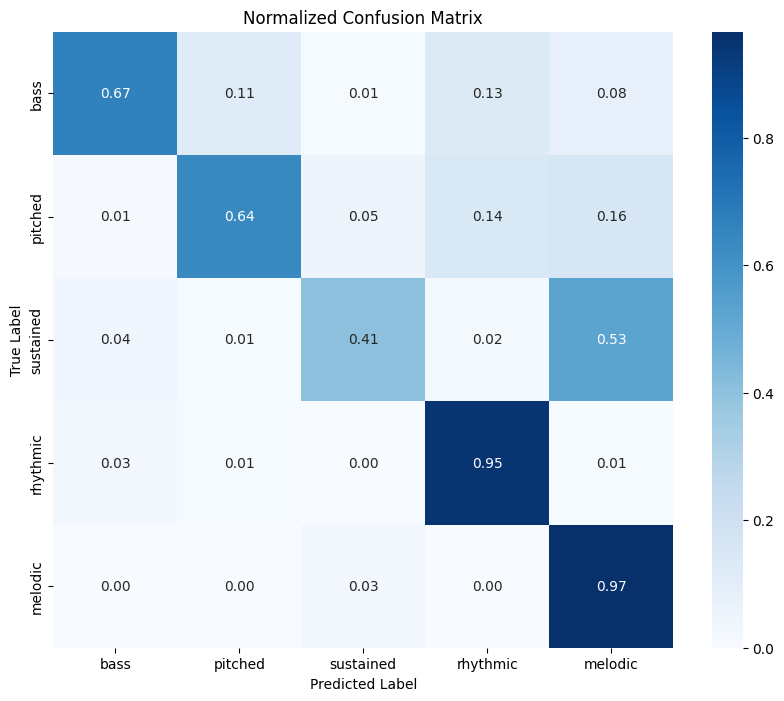
\includegraphics[width=0.65\textwidth]{images/10_test_validierung/nn/nn-confusion-matrix.png}
\caption{Confision-Matrix des trainierten neuronalen Netzes}
\label{fig:img-confusion-matrix}
\end{figure}

\end{adjustwidth}


\paragraph{Testfall: Überprüfen der Sinnhaftigkeit des Klassifikationsergebnisses}\mbox{}\\
\begin{adjustwidth}{0.5cm}{0cm}
\textbf{Schritte:}
\begin{enumerate}
	\item Es werden vier Audiosamples ermittelt, die nicht in den Trainingsdaten enthalten waren.
	\item Die Audiosamples werden wiedergegeben und notiert, welchen Merkmalsklassen sie jeweils zugeordnet sein sollten.
	\item Die fünf Audiosamples werden nacheinander mit dem Jupyter-Notebook ``ESP\_IMA\_validation`` klassifiziert.
	\item Die Klassifikationsergebnisse werden betrachtet und mit den notierten SOLL-Merkmalsklassen verglichen.
\end{enumerate}

\textbf{Erwartetes Ergebnis:} Die tatsächlichen Klassifikationsergebnisse (SOLL-Werte) decken sich mit den notierten Klassifikationsergebnissen (IST-Werte). Dabei wird ein Klassifikationsergebnis je Merkmalsklasse, das $\geq$ 0,5 ist, als ``erkannt`` gewertet.

\newpage

\textbf{Tatsächliches Ergebnis:}

1. Rock-Song

\begin{tabular}{|c|c|c|c|c|c|}
    \hline
    IST/SOLL & bass & pitched & rhythmic & sustained & melodic \\ \hline
    SOLL-Ausgabe & 0 & 0 & 1 & 0 & 1 \\ \hline
    IST-Ausgabe & 0.09 & 0.28 & 0.48 & 0.31 & 0.76 \\ \hline
\end{tabular}

2. Klaviermusik

\begin{tabular}{|c|c|c|c|c|c|}
    \hline
    IST/SOLL & bass & pitched & rhythmic & sustained & melodic \\ \hline
    SOLL-Ausgabe & 0 & 0 & 0 & 1 & 1 \\ \hline
    IST-Ausgabe & 0.14 & 0.14 & 0.01 & 0.85 & 0.92 \\ \hline
\end{tabular}

3. Schlagzeug-Solo

\begin{tabular}{|c|c|c|c|c|c|}
    \hline
    IST/SOLL & bass & pitched & rhythmic & sustained & melodic \\ \hline
    SOLL-Ausgabe & 0 & 0 & 1 & 0 & 0 \\ \hline
    IST-Ausgabe & 0.16 & 0.24 & 0.91 & 0.00 & 0.10 \\ \hline
\end{tabular}

4. Action-Song

\begin{tabular}{|c|c|c|c|c|c|}
    \hline
    IST/SOLL & bass & pitched & rhythmic & sustained & melodic \\ \hline
    SOLL-Ausgabe & 1 & 0 & 1 & 0 & 0 \\ \hline
    IST-Ausgabe & 0.41 & 0.23 & 0.97 & 0.03 & 0.36 \\ \hline
\end{tabular}

Wie in den Beispielen erkennbar ist, werden Merkmalsklassen nicht immer gut erkannt, jedoch lässt sich auch hier eine Tendenz ableiten. Beim Rock-Song beispielsweise liegt der Ähnlichkeitswert für die Klasse ``rhythmic`` mit 0,48 nur knapp unterhalb der Schwelle von 0,5. Beim Action-Song wird das Merkmal ``bass`` mit einer Ähnlichkeit von 0,41 erkannt, was auch nicht allzu weit weg ist vom Schwellenwert. Dennoch bleibt wie zuvor erwähnt nich Optimierungspotenzial mit mehr Trainingsdaten für bestimmte Klassen, um das Merkmalsspektrum besser abzubilden.

\end{adjustwidth}

%
%
%
%

\subsubsection{Validierung der korrekten Funktion der Klassifikation auf dem STM32 Microcontroller}
\paragraph{Testfall: Überprüfen der berechneten Spektrogramm-Werte}\mbox{}\\
\begin{adjustwidth}{0.5cm}{0cm}
\textbf{Schritte:}
\begin{enumerate}
	\item Ein Audiosample wird in das Jupyter-Notebook ``ESP\_IMA\_validation`` geladen und auf 16 kHz heruntergesampled.
	\item Die ersten 16.896 Samples (das erste Audiosubsample) des Audiosamples wird in Form von C-Code in Datei \mintinline{c}|test_audio_data.c| im CubeMX Projekt ``esp-cubeai-test`` geladen.
	\item Ein Breakpoint wird vor der Standardisierung der Eingabewerte gesetzt.
	\item Der Code wird via Debugger auf das Nucleo-Board geflashed.
	\item Es wird zu dem gesetzten Breakpoint gegangen und in CubemMX eine Expression für die Variable \mintinline{c}|spectrogram| gesetzt.
	\item Die Werte des Arrays werden mit den Spektrogramm-Werten des ersten Audiosubsamples im Jupyter-Notebook verglichen.
\end{enumerate}

\textbf{Erwartetes Ergebnis:} Es gibt keine bzw. kaum Abweichungen zwischen den Spektrogramm-Werten im Debugger  und den Werten aus dem Jupyter-Notebook.

\textbf{Tatsächliches Ergebnis:} Von den Werten 0 bis 700 wurden keine Abweichungen festgestellt. Nach diesem Bereich treten jedoch leichte Abweichungen auf. Diese können darauf zurückgeführt werden, dass die höheren Indizes des \mintinline{c}|spectrogram|-Arrays die Dezibel-Werte der höheren Frequenzbereiche enthalten. Es lässt sich daraus schließen, dass die verwendete Bibliothek zur Spektrogramm-Berechnung die höheren Frequenz-Werte anders skaliert. Insgesamt kann der Test mit einem positiven Ergebnis bewertet werden, wobei darauf hingewiesen werden muss, dass die leichten Abweichungen in der Spektrogramm-Berechnung zu geringfügigen Abweichungen in den Klassifikationsergebnissen führen könnten.
\end{adjustwidth}


\paragraph{Testfall: Überprüfen des Klassifikationsergebnisses}\mbox{}\\
\begin{adjustwidth}{0.5cm}{0cm}
\textbf{Schritte:}
\begin{enumerate}
	\item Ein Audiosample wird in das Jupyter-Notebook ``ESP\_IMA\_validation`` geladen und auf 16 kHz heruntergesampled.
	\item Die ersten 16.896 Samples (das erste Audiosubsample) des Audiosamples wird in Form von C-Code in Datei \mintinline{c}|test_audio_data.c| im CubeMX Projekt ``esp-cubeai-test`` geladen.
	\item Ein Breakpoint wird nach der Zeile des Funktionsaufrufs von \mintinline{c}|ai_network_1_run()| gesetzt.
	\item Der Code wird via Debugger auf das Nucleo-Board geflashed.
	\item Es wird zu dem gesetzten Breakpoint gegangen und in CubemMX eine Expression für die Variable \mintinline{c}|ai_out_data| gesetzt.
	\item Die Werte des Arrays werden mit dem Klassifikationsergebnis des ersten Audiosubsamples im Jupyter-Notebook verglichen.
\end{enumerate}

\textbf{Erwartetes Ergebnis:} Es gibt kaum Abweichungen zwischen den Werten im Debugger und den Werten aus dem Jupyter-Notebook. Eine geringe Abweichung ist zu erwarten, da wie im Ergebnis des vorherigen Testfalls beschrieben die berechneten Spektrogramm-Werte nicht identisch sind.


\textbf{Tatsächliches Ergebnis:}
Folgende IST-Werte wurden aus dem Debugger ausgelesen. Ein Screenshot Tabs ``Expressions``, in dem die Variableninhalte zur Laufzeit gezeigt werden, ist in \textbf{Abbildung \ref{fig:img-stm-classification-result}} zu sehen.

\begin{tabular}{|c|c|c|c|c|c|}
    \hline
    IST/SOLL & bass & pitched & sustained & rhythmic & melodic \\ \hline
    SOLL-Ausgabe & 0.12 & 0.28 & 0.06 & 0.93 & 0.37 \\ \hline
    IST-Ausgabe & 0.13 & 0.33 & 0.048 & 0.95 & 0.31 \\ \hline
\end{tabular}

Wie erwartet gibt es leichte Abweichungen im Klassifikationsergebnis. Dies ist wie zuvor erwähnt auf die abweichenden Spektrogramm-Werte zurückzuführen. Das Testergebnis ist als positiv zu beurteilen. 

\begin{figure}[h!]
\centering
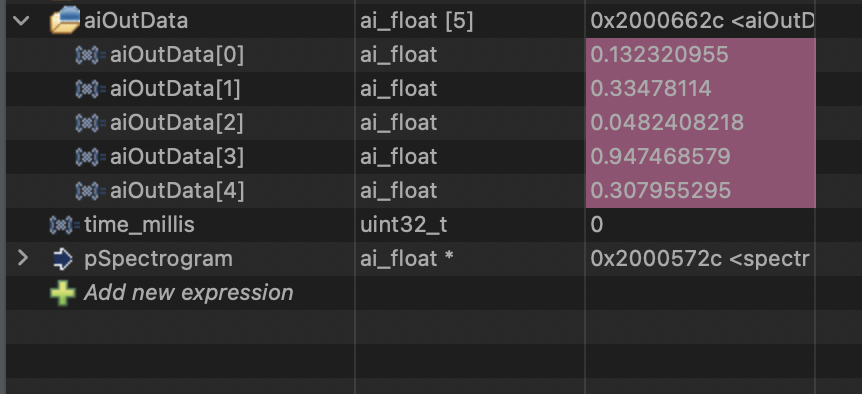
\includegraphics[width=0.45\textwidth]{images/10_test_validierung/nn/nn-debuger-classification-result.png}
\caption{Screenshot vom CubeAI Debugger. In den Elementen des ``aiOutData``-Arrays kann das Klassifikationsergebnis abgelesen werden.}
\label{fig:img-stm-classification-result}
\end{figure}

\end{adjustwidth}

